%#!platex -kanji=utf8 hb.tex
\chapter{執筆を始める前に}
% これはただのダミーテキスト.
% 文字コードを判定するための意味のない文字列.
% これくらい記述すれば大丈夫かな.
% Emacs のくせに生意気な.
% Emacs の分際で自動判別とか.
% Mac OS X のテキストエディッタの文字コード自動判別はうまくいかないぞ.

\section{\TeX と \LaTeX}
本書では\ruby{\LaTeX}{ラテック}と呼ばれる\W{文書執筆システム}のコマンドにつ
いて書式と入出力例を簡潔にまとめ,辞書として使いやすいようにまとめていま
す.科学技術系に限らず,ゼミのレジュメや学位論文,学会への投稿論文などに
使われているプログラムです.\LaTeX は通常のワープロソフトと違って,なれ
るまでに少々時間がかかる事があります.ある程度まとまった学習が必要になる
と思いますので『好き好き\LaTeXe 初級編』\cite{jou}など,一般に流通してい
る独習書をご参照ください.

\subsection{\TeX}
\index{TeX@\TeX}
\index{レイアウトとコンテンツの分離}
\ruby{\TeX}{テック}とはDonald Knuth氏によって開発された\LaTeX のベースと
なるシステムです.ただし,レイアウトとコンテンツを分離する記述の仕方では
ないため,直接\TeX を使うユーザは少数です.

\subsection{\LaTeX}
\index{LaTeX@\LaTeX}
\index{マークアップ言語}
\ruby{\LaTeX}{ラテック}とはLeslie Lamport氏によって構築されたマークアッ
プ版\TeX です.基本的なコンセプトとして,誰でも簡単にレイアウトの統一さ
れた文書を執筆できる環境を提供する事が挙げられます.\W{HTML}と同様に
\W{文書の構成要素}(文字や段落)にタグ(\W{メタ属性})を付与する記述
と書式が似ています.HTMLでは段落を中央揃えにするとき,(CSSなどを使わな
い場合,直接)次のように表記します.

\begin{intext}
<center>
  レイアウトとコンテンツを分離するような記述の仕
  方ではないため,直接TeX を使うユーザは少数です.
</center>
\end{intext}

\noindent
\LaTeX の場合はコマンドと呼ばれるHTMLのタグに相当する記述を
次のとおりに追加します.
\begin{intext}
\begin{center}
 レイアウトとコンテンツを分離するような記述の仕
 方ではないため,直接\TeX を使うユーザは少数です.
\end{center}
\end{intext}

また,\TeX/\LaTeX は欧文用に作られたシステムであるため,通常,日本語が
含まれる文章を執筆する時は,\W{アスキー}が開発した\pTeX ,または\pLaTeX
を使う事になります.

\index{LaTeX 2.09@\LaTeX\;2.09}
\index{LaTeX 2e@\LaTeXe}
\index{LaTeX 3@\LaTeX\;3}
\LaTeX は \LaTeX\;2.09からバージョンが上がり,現在\ruby{\LaTeXe}{ラテッ
ク・ツーイー}が使われています.将来的に\LaTeX\;3が配布される予定です.

\section{作業の進め方}
\LaTeX を用いてどのように原稿を執筆するかを説明します.

\subsection{全体の作業の流れ}
\index{GUIのワープロソフト}
\index{WIMP}
\index{全体の処理の流れ}
\index{執筆の進め方}
\TeX/\LaTeX はGUIのワープロソフトと違い,\W{バッチ処理}(一括処理)を採
用しているシステムです.WIMP(ウィンドウ,アイコン,マウス,ポインタ)のメタファも持ち
合わせていません.すなわち,\W{テキストエディッタ}などによって原稿を執筆し,
それを\W{成形}(\W{タイプセット}または\W{コンパイル}とも言います)する作業を行います.
全体の作業の流れを\figref{作業の流れ}に示します.

\begin{figure}[htbp]
 \centering
 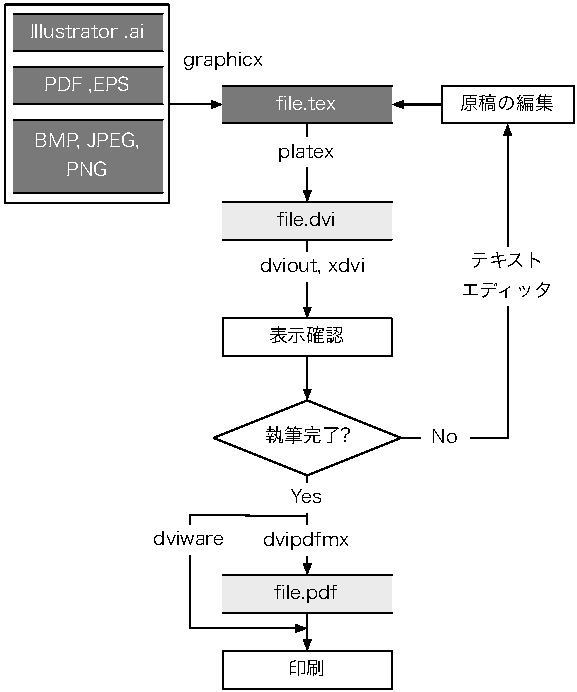
\includegraphics{process}
 \caption{作業の流れ}\figlab{作業の流れ}
\end{figure}

\index{原稿}%
\zindind{原稿}{の編集}%
\zindind{ソースファイル}{の編集}%
\index{編集}%
\indindz{編集}{原稿の}%
\indindz{編集}{ソースファイルの}%
ユーザが編集すべきファイルは濃いグレーで示してあります.画像ファイルと原
稿である\fl{file.tex}を編集し,これを日本語化された\LaTeX である
\W{platex}コマンドで成形します.

成形結果は\fl{file.dvi}というファイルに書き出される事になります.この
成形結果を見るために\W{プレビューア}と呼ばれるソフトウェアを使って表示を
確認します.

\index{dvipdfm}%
\index{ebb}%
文書の執筆が完了したら\W{dvipdfmx}によりPDFに変換し,印刷や配布を行う形
になると思います.Unix系OSに限りませんが\W{PostScript}ファイルへ変換する
ために\W{dvips}も使えます.

dvipdfmxは\Person{Mark}{Wicks}が開発したdvipdfmを\hito{平田}{俊作}と
\Hito{趙}{珍煥}が改良したものです.dvipdfmxではPDFの暗号化や
\W{単一ページのPDF},\W{PNG},\W{JPEG},Windows~\W{BMP}画像に対応してい
ます(ただし,これらの画像は\W{BoundingBox}と呼ばれる画像の領域情報が必
要になります.ebbコマンドにより\val{画像}\fl{.png}から\val{画像}\fl{.bb}
を作成する事でBoundingBox情報を作成する事も出来ますし,\Y{mediabb}パッケー
ジ\footnote{\webMediaBB}により自動的に生成可能です).

platexというコマンド一つを実行するだけで,全ての工程を完了できる訳ではな
く,複数のコマンドを実行する事で所望の文書・出力結果が得られる事になりま
す.これらの作業を簡略化するために,各種のOSにおいてGUIの執筆支援プログ
ラムが存在します.


\subsection{\pLaTeX の動かし方}
原稿となる\fl{file.tex}から成形後の\fl{file.dvi}を作成するためには
platexコマンドを実行します.動作イメージを\figref{platexの動作イメージ}
に示します.近年はplatexコマンド以外にも直接PDFを出力する\PDFLaTeX や,
Unicodeに対応した\upTeX などが開発されていますが,これらについては
\appref{ヒントと今後の動向}を参照して下さい.platexコマンドを実行するに
は\fl{file.tex}以外にも実に様々なファイルが必要になります.フォント情報
が記述されたファイル (.fmt, .tfm, .fd),文書の書式を決定するクラスファイ
ル (.cls),様々な機能を提供するマクロパッケージ (.sty) などが挙げられま
す.

%\PDFTeX by \Person{H\`an Th\'{\^e}}{Th\`anh}

\begin{figure}[htbp]
 \centering
 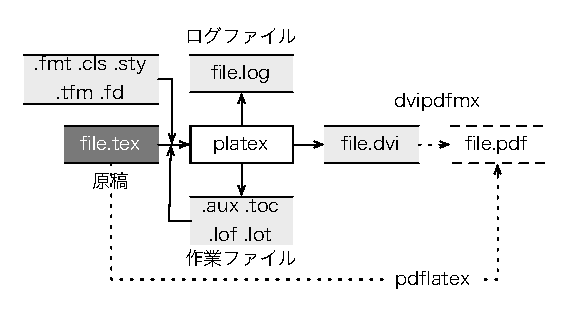
\includegraphics{process-latex}
 \caption{platexの動作イメージ}\figlab{platexの動作イメージ}
\end{figure}

実際にplatexコマンドを実行すると,\LaTeX 自身が必要とする作業ファイル
(.aux, .toc, .lof, .lot) が出力されます.そして,処理の結果をログファイ
ル \fl{file.log}に書き出します.

\subsection{\JBibTeX の動かし方}
\index{BibTeX@\BibTeX}
\index{JBibTeX@\JBibTeX}
論文などでは文献を引用した場合,参考文献の一覧を載せることになっています.
提出先によって異なりますが,大抵は一定のルールに則り並び替えたり,表記を
統一する必要があります.これらの作業を手動で行う事も可能ですが,並び替え
や表記の統一を行うプログラムが\LaTeX では提供されています.それがOren
Patashnik氏が作成した\BibTeX と呼ばれるプログラムです.日本語が含まれて
いる場合は日本語化された{\JBibTeX} (jbibtex) を使う事になります.の{\JBibTeX}
動作イメージを\figref{jbibtexの動作イメージ}に示します.
\begin{figure}[htbp]
 \centering
 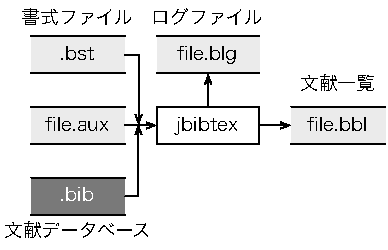
\includegraphics{process-bibtex}
 \caption{jbibtexの動作イメージ}\figlab{jbibtexの動作イメージ}
\end{figure}
\index{BibTeX@\BibTeX!スタイルファイル@\zdash スタイルファイル}
これは{\LaTeX} (platexコマンドなど) が書き出した作業ファイル
(\fl{file.aux}) と,ユーザが作成する\W{文献データベース} .bib,並びに文
献一覧のスタイルを決定するファイル (.bst) を入力とするものです.成形後の
文献一覧がファイル \fl{file.bbl} に書き出されます.文法的なエラーが発生
した場合などはログファイル\fl{file.blg}を参照します.

\JBibTeX が作成した\W{文献一覧ファイル} \fl{file.bbl} では\W{相互参照}と
いう機能が使われていますので,必要に応じて複数回platexコマンドを実行する
ことになります.

\section{\LaTeX の導入}
\index{GUIによるインストール}
\index{インストーラによるTeXの導入@インストーラによる\TeX の導入}
\LaTeX を使うためにはplatexコマンドが一つあれば良いという訳ではなく,複
数のプログラム,設定ファイル,フォント関連ファイルが必要になります.
これらを適切な場所に適切な配置でシステムにインストールします.そのため,
主要なファイルを収録したディストリビューションがいくつか存在します.また,
コマンドラインからの操作によるインストールが主流でしたが,
近年はWindows,Mac OS X,Linuxにおける\TeX/\LaTeX のGUIインストーラで
導入できるようになりました.本書では詳しく述べる事が出来ませんが,ウェブ
上の解説ページを参照ください.
執筆環境に関してもテキストエディタのみで行う事も可能ですが,Windowsであ
れば{Easy\TeX},Mac~OS~Xであれば\TeX Shop を使用する事ができます.


\section{サンプルの実行の仕方}
\index{標準のコマンド}
本書では各種コマンドの用例を示してありますが,実際に\LaTeX プログラムで
処理するためには最低限,以下の記述が必要です.

\begin{intext}
\documentclass{jsarticle}
\begin{document}
ここに文章・用例を記述します
\end{document}
\end{intext}

\subsection{環境と命令}
\index{環境}%
\index{命令}%
\LaTeX のコマンドを大別すると『環境』と『命令』の二つに別れます.
命令は引数を取る場合もありますし,取らない場合もあります.
以下は引数を取る命令の例です.

\begin{intext}
\documentclass{jsarticle}
\end{intext}

環境は `\verb|\begin|\param{環境名}' で始まり,`\verb|\end|\param{環境名}'
で終わるコマンドです.以下は引数を取らない環境の例です.

\begin{intext}
\begin{center}
 この部分が中央揃えになります.
\end{center}
\end{intext}

\subsection{用例中の必須引数と任意引数}
\index{引数}%
\index{必須引数}%
\index{任意引数}%
\LaTeX コマンドは単なる宣言として使うものもありますが,多くの命令や環境
の中には『引数』を取るものがあります.必ず引数が必要なものは,波括弧を
用いて `\param{必須引数}' と用例で記述しています.任意の引数は角括弧を用いて
`\opt{任意引数}' のように記述しています.

例えば, \cmd{documentclass} 命令は任意引数に \opt{クラスオプション},
必須引数に \param{クラス名} を取ります.

\begin{usage}
\documentclass[$\<クラスオプション>$]{$\<クラス名>$}
\end{usage}

クラスに`\cls{jsarticle}'を用いており,オプションに`\option{a4j}'と
`\option{twocolumn}'を指定したい場合,具体的には次のように記述します.
\begin{intext}
\documentclass[a4j,twocolumn]{jsarticle} 
\end{intext}
任意引数はカンマ区切りで複数指定する事が出来ます.ただし,コマンドによっ
ては競合するために同時に指定する事が出来ないものもあります.


\subsection{マクロパッケージの活用}
\index{パッケージ}%
\zindind{原稿}{の編集}%
\zindind{パッケージ}{を読み込む}%
\zindind{マクロパッケージ}{を読み込む}%
\latexno{の機能を拡張する}%
\LaTeX には標準的なコマンド以外にも\W{マクロパッケージ}と呼ばれるファイ
ルを読み込む事で機能を拡張する事が出来ます.パッケージを読み込むに
は \C{usepackage} 命令を \verb|\begin{document}| よりも前の部分(\W{プリアンブ
 ル})に追加します.

\begin{intext}
\documentclass{jsarticle}
\usepackage[dvipdfmx]{color,graphicx}
\begin{document} 
\end{intext}

ほとんどのパッケージはCTANと呼ばれる集約サイトで入手する事ができます.一
部著者のオリジナルが含まれています.

本書をタイプセットするために必要となるマクロ・パッケージの所在については,
サポートページ\footnote{\webMyTeXpert}で配布する原稿中の
 \fl{mcr/required.ltx}に全て書かれていますので,そちらをご参照ください.
 

\subsection{jsclasses}
\index{TeXインストーラ3@\TeX インストーラ3}
用例に何ら記述がされていない場合でも,
奥村晴彦氏による
\Cls{jsclasses}\footnote{\webJsclasses}を文書クラスファイルに指定する事を前提にし
ています.アスキーによる\Y{jclasses}と比較して各種改良が施されていますの
で,インストールする事をおすすめします.\W{ptetex3}\footnote{\webPtetex}には
既に含まれており,阿部紀行氏による『\TeX インストーラ3』
\footnote{\webTeXInstaller}ではインストール時の選択で導入可能です.
\cls{jsclasses}は\Cls{jsarticle}と\Cls{jsbook}の二つのクラス,
\Y{okumacro}というパッケージを総称したものです.

% jarticle はやめて jsarticle を使おう運動
% 歴史的諸事情により使わざるを得ない場合があるだろう

%\subsection{バックスラッシュと円記号}

\subsection{そのまま出力できない記号}
{\LaTeX}では\Z{予約文字}と呼ばれる以下の13個の半角記号を直接出力できませ
ん.
\begin{quote}
 \verb+\ { } $ & # ^ _ ~ % < > |+
\end{quote}
%の13個であり,それらの記号を出力するには付録を参照してください.
また,Windowsの場合はバックスラッシュを半角の円記号`\textyen'と読み替え
てください.Mac~OS~XやLinuxの場合は通常通り,半角のバックスラッシュ`\BS'
を入力してください.

\subsection{ソースファイルの全体像}
以下に簡単な原稿の入力例を示します.\figref{コマンドと出力例の併合}が出
力イメージになります.
\begin{intext}
\documentclass{jsarticle}
\title{\LaTeXe 入門}%  題名
\author{A. U. Th\'or}% 著者
\date{\today}%         日付
\begin{document}%      本文
\maketitle%            表紙
\tableofcontents%      目次
\section{節見出し}%       節見出し
節見出しは \verb|\section| コマンドを使います。
\subsection{小節見出し}%  小節見出し
小節見出しは \verb|\subsection| を使います。
\section{文章の記述}
この節では文章の記述について論じます。
\subsection{引用}
一文を引用する場合はカギ括弧を使います。一説によると
「カギ括弧は引用に使う」と言われている。
段落ごと引用するということは次のようになっている。
\begin{quote}
一つの段落の引用の場合は \verb|quote| 環境を使い、
\emph{行頭を字下げしない}のが普通である。複数段落の引用
の場合は \verb|quotation| 環境を使い、行頭を字下げする。
\end{quote}
\subsection{箇条書き}
箇条書きには以下の三つが用意されている。
\begin{description}
 \item[記号付箇条書き] ラベルの先頭に記号がついた箇条書き。
 \item[番号付箇条書き] ラベルの先頭に番号がついた箇条書き。
 \item[説明付箇条書き] ラベルの先頭に説明がついた箇条書き。
\end{description}
\end{document}	
\end{intext}

\begin{figure}[htbp]
 \begin{center}
  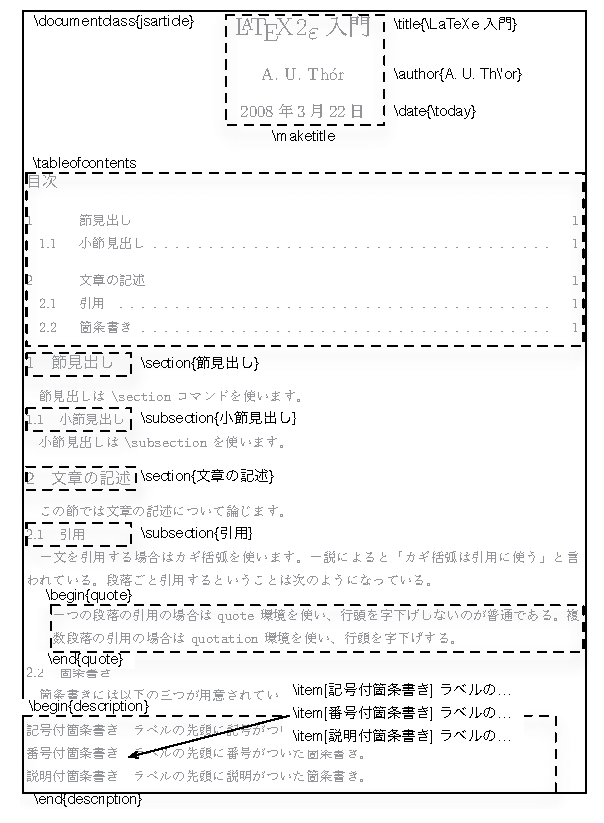
\includegraphics{sample-cmd}
  \caption{\LaTeX コマンドと出力例の併合}\figlab{コマンドと出力例の併合}
 \end{center}
\end{figure}


